\section{Beyond Physical Memory: Policies}

%------------------------------------------------
\begin{frame}{Memory Pressure and Replacement}

\begin{itemize}
    \item With lots of free memory: page fault $\rightarrow$ take a page from
          the \textbf{free-page list}.
    \item With little free memory, \textbf{memory pressure} forces the OS to
          page out pages to make room for actively-used ones.
    \item Deciding which page(s) to evict: the \textbf{replacement policy}.
\end{itemize}

\begin{block}{Crux: How to Decide Which Page to Evict}
How can the OS decide which page (or pages) to evict from memory? The
replacement policy usually follows general principles but also includes
tweaks to avoid corner-case behaviors.
\end{block}

\end{frame}

%------------------------------------------------
\begin{frame}{Cache Management}

\begin{itemize}
    \item Main memory as a \textbf{cache} for virtual memory pages.
    \item Goal: \textbf{minimize cache misses} (maximize cache hits).
    \item \textbf{Average memory access time}:
\end{itemize}

\begin{equation*}
    AMAT = T_M + (P_{Miss} \cdot T_D)
\end{equation*}

\begin{itemize}
    \item Example: $T_M = 100$\,ns, $T_D = 10$\,ms:
    \begin{itemize}
        \item 90\% hit rate ($P_{Miss}=0.1$): AMAT $\approx$ \textbf{1\,ms};
        \item 99.9\% hit rate ($P_{Miss}=0.001$): AMAT $\approx$
              \textbf{10.1\,$\mu$s} (about 100 times faster).
    \end{itemize}
    \item Disk access cost is so high that even a \textbf{tiny miss rate}
          dominates the AMAT.
\end{itemize}

\end{frame}

%------------------------------------------------
\begin{frame}{The Optimal Replacement Policy}

\begin{columns}[T]

\column{0.50\textwidth}
\small
\begin{itemize}
    \item Belady's \textbf{MIN}: replace the page that will be accessed
          \textbf{furthest in the future}.
    \item Fewest possible misses, but the future is generally unknown:
          useful only as a \textbf{comparison point}.
    \item Stream \texttt{0,1,2,0,1,3,0,3,1,2,1}, 3-page cache:
          6 hits, 5 misses $\Rightarrow$ \textbf{54.5\%}
          (85.7\% ignoring compulsory misses).
\end{itemize}

\column{0.48\textwidth}
\begin{figure}
    \centering
    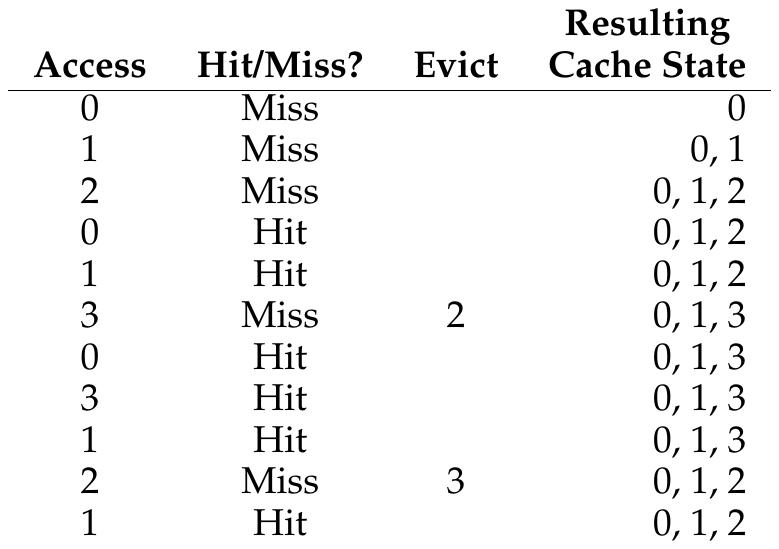
\includegraphics[height=0.40\textheight]{figs/chapter-22/figure-22.1.png}
    \caption*{Source: chapter page 3.}
    \label{fig:figure-22.1}
\end{figure}

\end{columns}

\begin{block}{Tip: Comparing Against Optimal Is Useful}
Knowing the optimal shows how much improvement is still possible, and
when a policy is close enough to the ideal.
\end{block}

\end{frame}

%------------------------------------------------
\begin{frame}{Types of Cache Misses}

\begin{itemize}
    \item The \textbf{Three C's}:
    \begin{itemize}
        \item \textbf{compulsory} (cold-start): cache empty, first reference
              to the item;
        \item \textbf{capacity}: the cache ran out of space and had to evict;
        \item \textbf{conflict}: limits on where an item can be placed
              (set-associativity) in hardware caches.
    \end{itemize}
    \item The OS page cache is \textbf{fully-associative}: no conflict misses.
\end{itemize}

\end{frame}

%------------------------------------------------
\begin{frame}{A Simple Policy: FIFO}

\begin{columns}[T]

\column{0.50\textwidth}
\small
\begin{itemize}
    \item Pages enter a \textbf{queue}; evict the ``first-in'' page.
    \item Strength: very \textbf{simple to implement}.
    \item Hit rate \textbf{36.4\%} (57.1\% excluding compulsory misses).
    \item Cannot determine the \textbf{importance} of pages: page 0 is evicted
          even though it was accessed many times.
\end{itemize}

\column{0.48\textwidth}
\begin{figure}
    \centering
    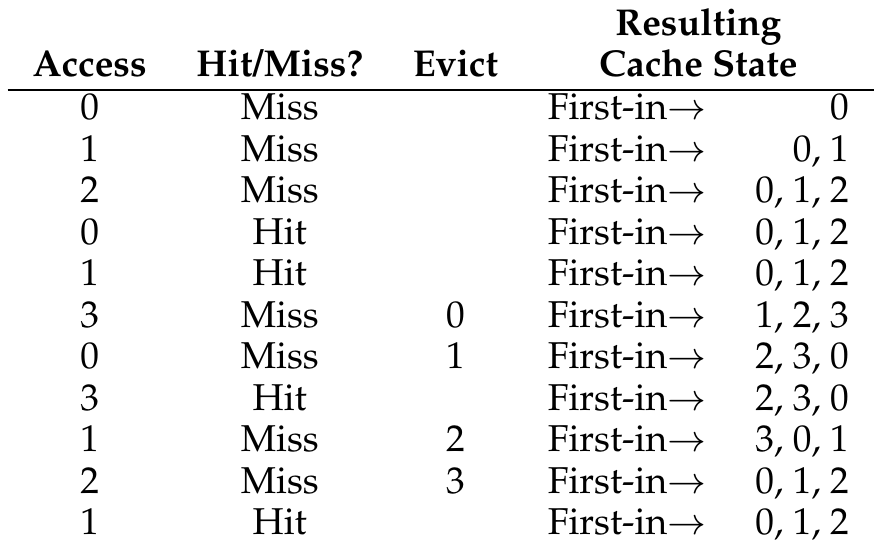
\includegraphics[width=\linewidth,height=0.55\textheight,keepaspectratio]{figs/chapter-22/figure-22.2.png}
    \caption*{Source: chapter page 5.}
    \label{fig:figure-22.2}
\end{figure}

\end{columns}

\end{frame}

%------------------------------------------------
\begin{frame}{Belady's Anomaly}

\begin{itemize}
    \item Stream: \texttt{1,2,3,4,1,2,5,1,2,3,4,5} with FIFO.
    \item Moving from a cache of \textbf{3 to 4 pages}, the hit rate
          gets \textbf{worse}!
    \item LRU has the \textbf{stack property}: a cache of size $N+1$ naturally
          includes the contents of a cache of size $N$.
    \item FIFO and Random do not obey the stack property and are
          susceptible to anomalous behavior.
\end{itemize}

\end{frame}

%------------------------------------------------
\begin{frame}{Another Simple Policy: Random}

\begin{columns}[T]
\column{0.48\textwidth}
\begin{figure}
    \centering
    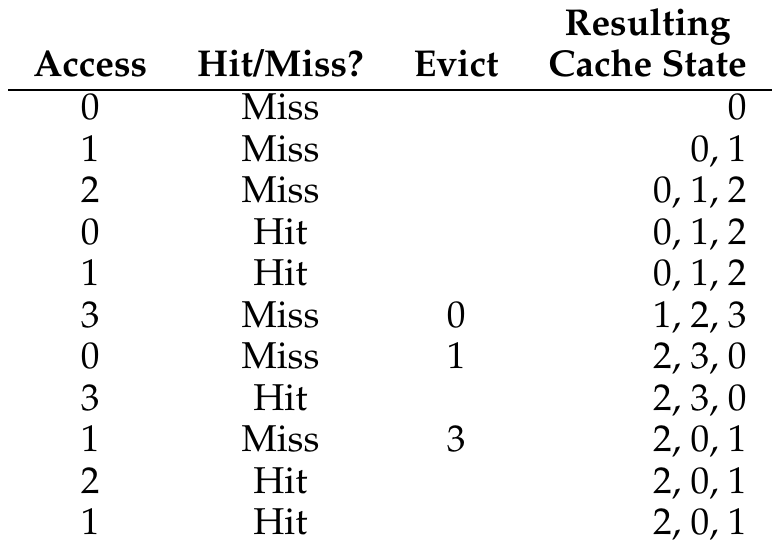
\includegraphics[width=0.95\linewidth]{figs/chapter-22/figure-22.3.png}
    \caption*{Source: chapter page 6.}
    \label{fig:figure-22.3}
\end{figure}
\column{0.50\textwidth}
\begin{figure}
    \centering
    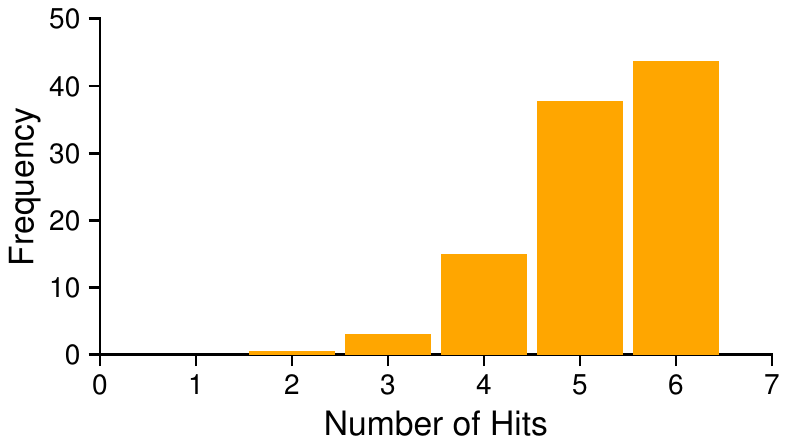
\includegraphics[width=0.95\linewidth]{figs/chapter-22/figure-22.4.png}
    \caption*{Source: chapter page 6.}
    \label{fig:figure-22.4}
\end{figure}
\end{columns}

\begin{itemize}
    \item Picks a \textbf{random page} to replace: simple, but not intelligent.
    \item Depends on luck: over 10,000 trials, just over 40\% of the time it
          is as good as optimal (6 hits); sometimes 2 hits or fewer.
\end{itemize}

\end{frame}

%------------------------------------------------
\begin{frame}{Using History: LRU}

\begin{columns}[T]

\column{0.50\textwidth}
\small
\begin{itemize}
    \item Use the past as a guide: \textbf{frequency} or
          \textbf{recency} of access.
    \item Based on the \textbf{principle of locality}.
    \item \textbf{LFU}: evicts the least-frequently-used page.
    \item \textbf{LRU}: evicts the least-recently-used page.
    \item On the example, LRU \textbf{matches optimal}.
    \item Opposites (MFU, MRU) usually work poorly: they ignore locality.
\end{itemize}

\column{0.48\textwidth}
\begin{figure}
    \centering
    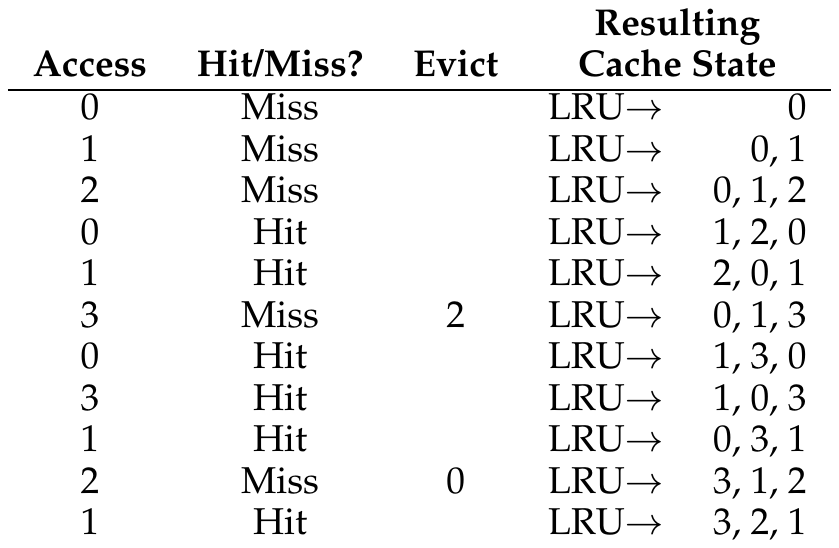
\includegraphics[width=\linewidth,height=0.55\textheight,keepaspectratio]{figs/chapter-22/figure-22.5.png}
    \caption*{Source: chapter page 7.}
    \label{fig:figure-22.5}
\end{figure}

\end{columns}

\end{frame}

%------------------------------------------------
\begin{frame}{Types of Locality}

\begin{itemize}
    \item \textbf{Spatial locality}: if page $P$ is accessed, pages around it
          ($P-1$, $P+1$) are likely to be accessed.
    \item \textbf{Temporal locality}: pages accessed in the near past are
          likely to be accessed again in the near future.
    \item Hardware caching hierarchies rely heavily on these assumptions.
    \item Locality is \textbf{no hard-and-fast rule}: some programs access
          memory randomly. It is a useful \textbf{heuristic}, not a guarantee.
\end{itemize}

\end{frame}

%------------------------------------------------
\begin{frame}{Workload Examples: No Locality and 80-20}

\begin{columns}[T]
\column{0.48\textwidth}
\begin{figure}
    \centering
    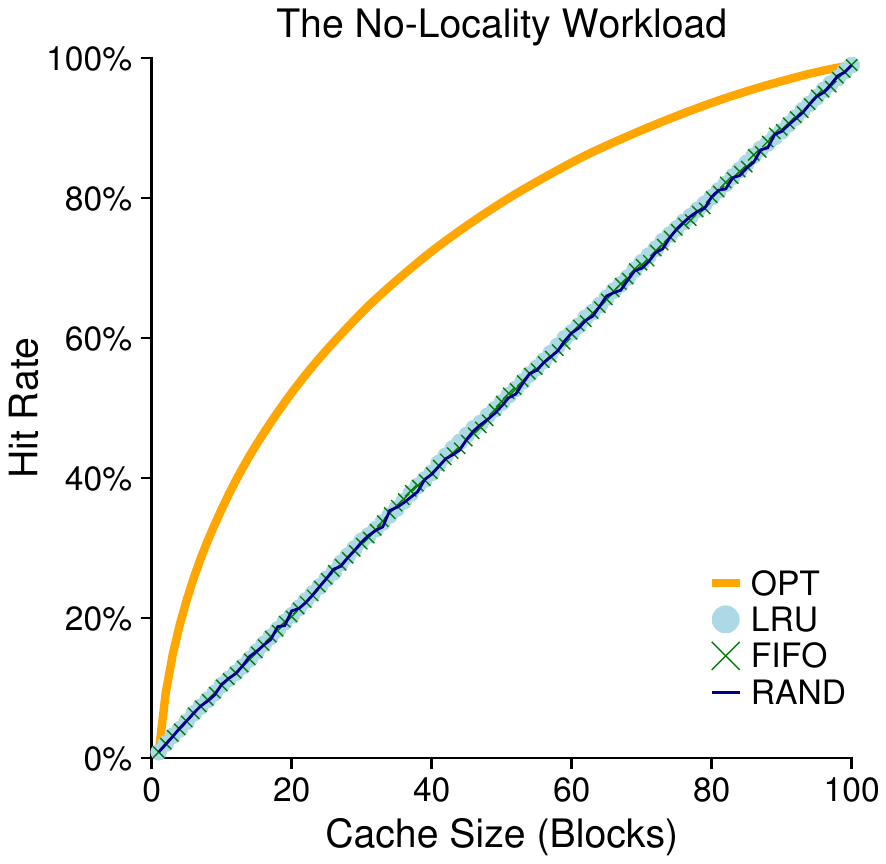
\includegraphics[height=0.38\textheight]{figs/chapter-22/figure-22.6.png}
    \caption*{Source: chapter page 9.}
    \label{fig:figure-22.6}
\end{figure}
\column{0.48\textwidth}
\begin{figure}
    \centering
    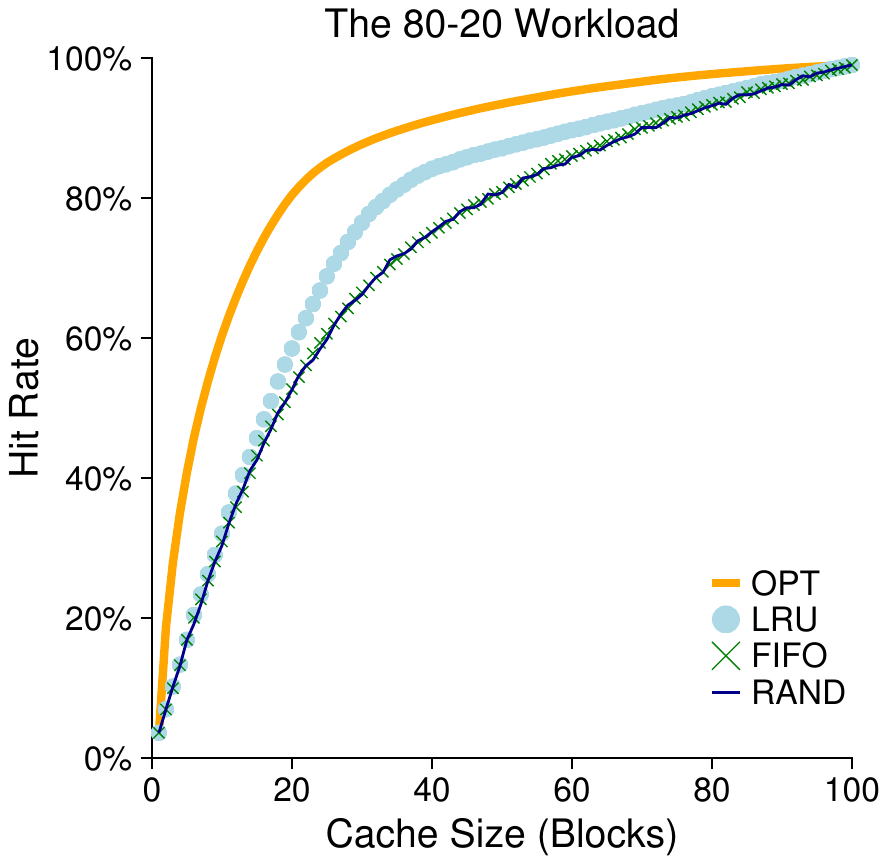
\includegraphics[height=0.38\textheight]{figs/chapter-22/figure-22.7.png}
    \caption*{Source: chapter page 10.}
    \label{fig:figure-22.7}
\end{figure}
\end{columns}

{\small
\begin{itemize}
    \item \textbf{No locality} (100 pages, 10,000 random accesses): realistic
          policies perform the same; hit rate set by cache size; all reach
          100\% when everything fits; OPT is noticeably better.
    \item \textbf{80-20} (80\% of refs to 20\% ``hot'' pages): LRU does better
          by holding onto hot pages. Whether it matters depends on the
          \textbf{cost of a miss}.
\end{itemize}
}

\end{frame}

%------------------------------------------------
\begin{frame}{Workload Examples: Looping Sequential}

\begin{columns}[T]

\column{0.50\textwidth}
\small
\begin{itemize}
    \item 50 pages accessed in sequence, repeatedly (10,000 accesses).
    \item Common in applications such as \textbf{databases}.
    \item \textbf{Worst case} for LRU and FIFO: they evict older pages that
          will be accessed sooner.
    \item Even with a 49-page cache: \textbf{0\% hit rate}.
    \item Random fares better: no weird corner-case behaviors.
\end{itemize}

\column{0.48\textwidth}
\begin{figure}
    \centering
    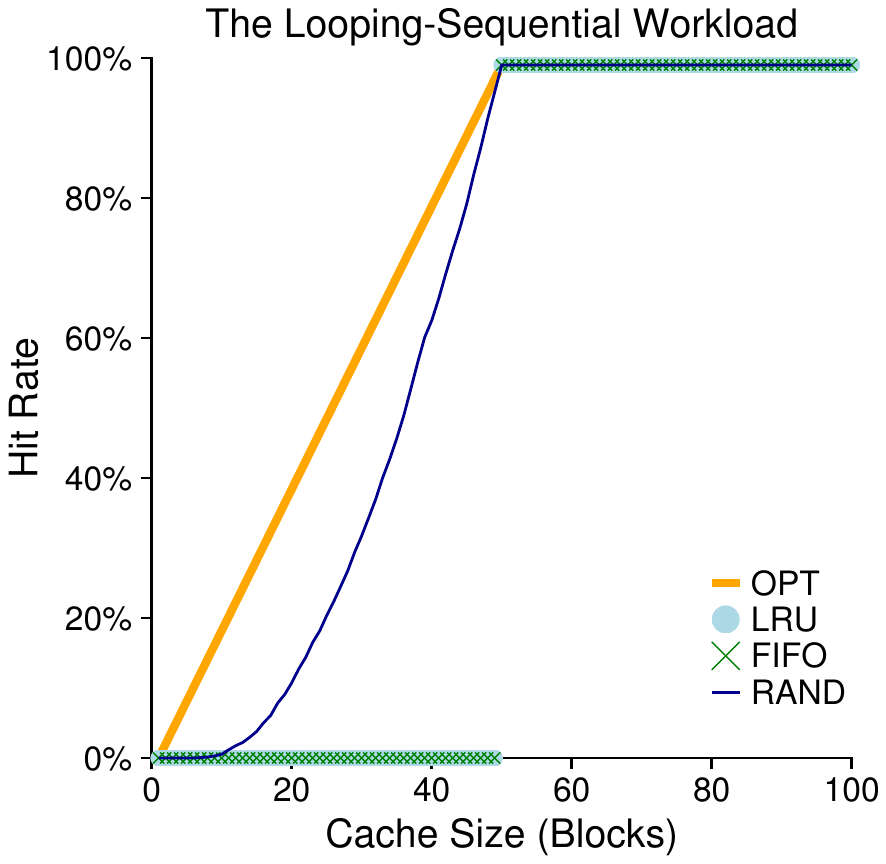
\includegraphics[width=\linewidth,height=0.55\textheight,keepaspectratio]{figs/chapter-22/figure-22.8.png}
    \caption*{Source: chapter page 11.}
    \label{fig:figure-22.8}
\end{figure}

\end{columns}

\end{frame}

%------------------------------------------------
\begin{frame}{Implementing Historical Algorithms}

\begin{itemize}
    \item Perfect LRU: update a data structure on \textbf{every memory
          reference} (move page to the MRU side).
    \item FIFO touches its list only on eviction or insertion.
    \item Hardware help: a \textbf{time field} per page, set on each access;
          the OS scans all fields to find the LRU page.
    \item Problem: 4GB of memory with 4KB pages = \textbf{1 million pages}
          to scan: prohibitively expensive.
\end{itemize}

\begin{block}{Crux: How to Implement an LRU Replacement Policy}
Given that it will be expensive to implement perfect LRU, can we
approximate it in some way, and still obtain the desired behavior?
\end{block}

\end{frame}

%------------------------------------------------
\begin{frame}{Approximating LRU: The Clock Algorithm}

\begin{columns}[T]

\column{0.52\textwidth}
\small
\begin{itemize}
    \item Hardware \textbf{use bit} (reference bit), first in the Atlas
          one-level store: set to 1 on each access; cleared only by the OS.
    \item \textbf{Clock}: pages in a circular list; the hand checks page $P$:
    \begin{itemize}
        \item use bit 1 $\rightarrow$ clear it and advance;
        \item use bit 0 $\rightarrow$ \textbf{evict} $P$.
    \end{itemize}
    \item Does not repeatedly scan all of memory.
    \item Not as good as perfect LRU, but better than policies without
          history.
\end{itemize}

\column{0.46\textwidth}
\begin{figure}
    \centering
    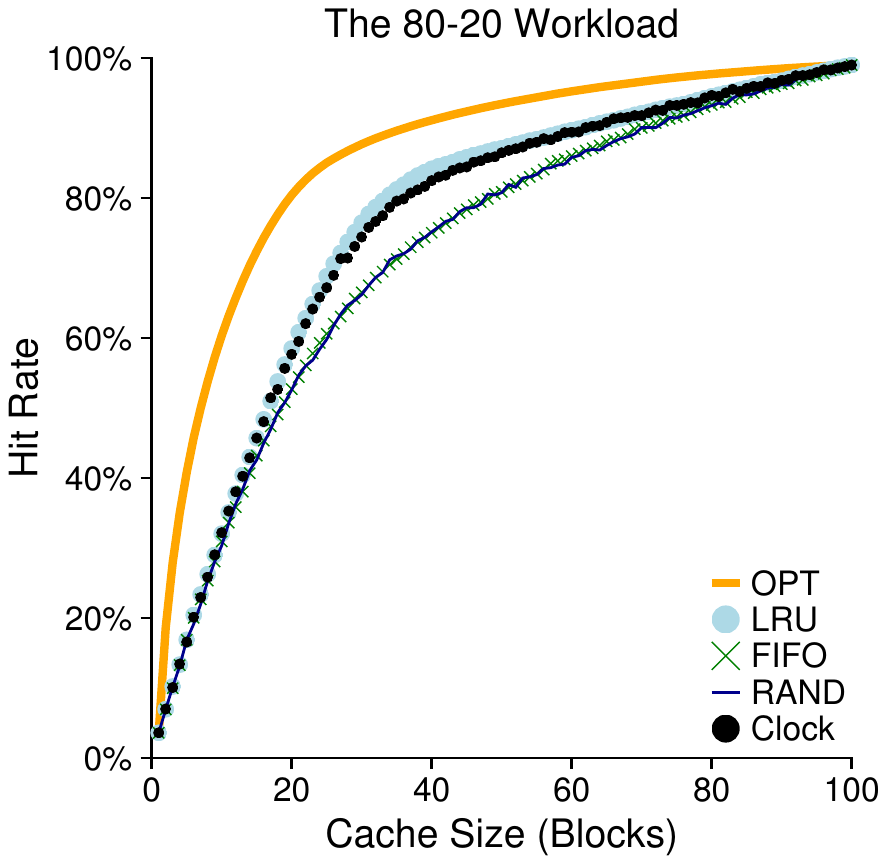
\includegraphics[width=\linewidth,height=0.55\textheight,keepaspectratio]{figs/chapter-22/figure-22.9.png}
    \caption*{Source: chapter page 13.}
    \label{fig:figure-22.9}
\end{figure}

\end{columns}

\end{frame}

%------------------------------------------------
\begin{frame}{Considering Dirty Pages}

\begin{itemize}
    \item A \textbf{dirty} (modified) page must be written back to disk
          before eviction: expensive.
    \item A \textbf{clean} page can be evicted for free (no extra I/O).
    \item Hardware \textbf{modified bit} (dirty bit), set on every write.
    \item Modified clock: evict pages that are \textbf{unused and clean}
          first; then unused and dirty, and so forth.
\end{itemize}

\end{frame}

%------------------------------------------------
\begin{frame}{Other VM Policies}

\begin{itemize}
    \item \textbf{Page selection policy}: when to bring a page into memory.
    \begin{itemize}
        \item \textbf{Demand paging}: bring the page in when it is accessed;
        \item \textbf{Prefetching}: bring it in ahead of time when success is
              likely (e.g., code page $P+1$ after $P$).
    \end{itemize}
    \item How to write pages out to disk:
    \begin{itemize}
        \item \textbf{clustering} (grouping) of pending writes into one large,
              more efficient write.
    \end{itemize}
\end{itemize}

\end{frame}

%------------------------------------------------
\begin{frame}{Thrashing}

\begin{itemize}
    \item Memory demands of running processes \textbf{exceed} physical
          memory $\Rightarrow$ constant paging: \textbf{thrashing}.
    \item \textbf{Admission control}: do not run a subset of processes, so
          the remaining \textbf{working sets} fit in memory.
    \begin{itemize}
        \item Better to do less work well than everything poorly.
    \end{itemize}
    \item More draconian: some versions of Linux run an
          \textbf{out-of-memory killer} that kills a memory-intensive process
          (may kill, e.g., the X server).
\end{itemize}

\end{frame}

%------------------------------------------------
\begin{frame}{Summary}

\begin{itemize}
    \item Page replacement (and other) policies are part of the VM subsystem
          of all modern OSes.
    \item Modern systems tweak LRU approximations such as clock; e.g.,
          \textbf{scan resistance} (ARC) avoids LRU's looping worst case.
    \item For years, disk was so slow that the best solution was:
          \textbf{buy more memory}.
    \item Faster storage (Flash-based SSDs) has led to a
          \textbf{renaissance} in page-replacement algorithms.
\end{itemize}

\end{frame}

%------------------------------------------------
\begin{frame}{Homework (Simulation)}

\begin{itemize}
    \item Simulator: \texttt{paging-policy.py}.
    \item Traces with \texttt{-s 0/1/2 -n 10}: compute hits and misses
          under FIFO, LRU and OPT.
    \item For a cache of size 5, generate worst-case streams for FIFO, LRU and
          MRU. How much bigger must the cache be to approach OPT?
    \item Random trace vs. trace with locality: how do LRU, RAND and CLOCK
          (with different numbers of clock bits) perform?
    \item Use \texttt{valgrind --tool=lackey --trace-mem=yes} to trace a real
          application and plot its working set versus cache size.
\end{itemize}

\end{frame}
